\chapter*{Dicom-Presenter}
\addcontentsline{toc}{chapter}{Dicom-Presenter}
\vspace{-10mm}

My predecessor Bc. Pavel Neskudla started development of an application for viewing images from MRI as a part of his master's thesis\cite{neskudla}. It was a task given by IKEM institute in Prague\footnote{Institute for Clinical and Experimental Medicine}. IKEM institute specialists found out that they would utilize some application which would allow them to open MRI images elsewhere than only on Siemens computers located in their institute. They would prefer some application where they could view recorded images on their own personal computers. It is possible to find such applications distributed by local developers, but only a few of them reach satisfactory quality requirements. These are definitely commercial applications, so user has to pay. There is also a lot of non-commercial, freeware applications, but functionality of these applications is often limited\cite[page~9]{flaska_bc}. For example, it was not possible to find an application which could open several images at the same time and view them on one screen. Therefore, specialists from IKEM institute decided to ask our faculty to develop such an application which would fit their needs.

\begin{figure}
	\begin{center}
	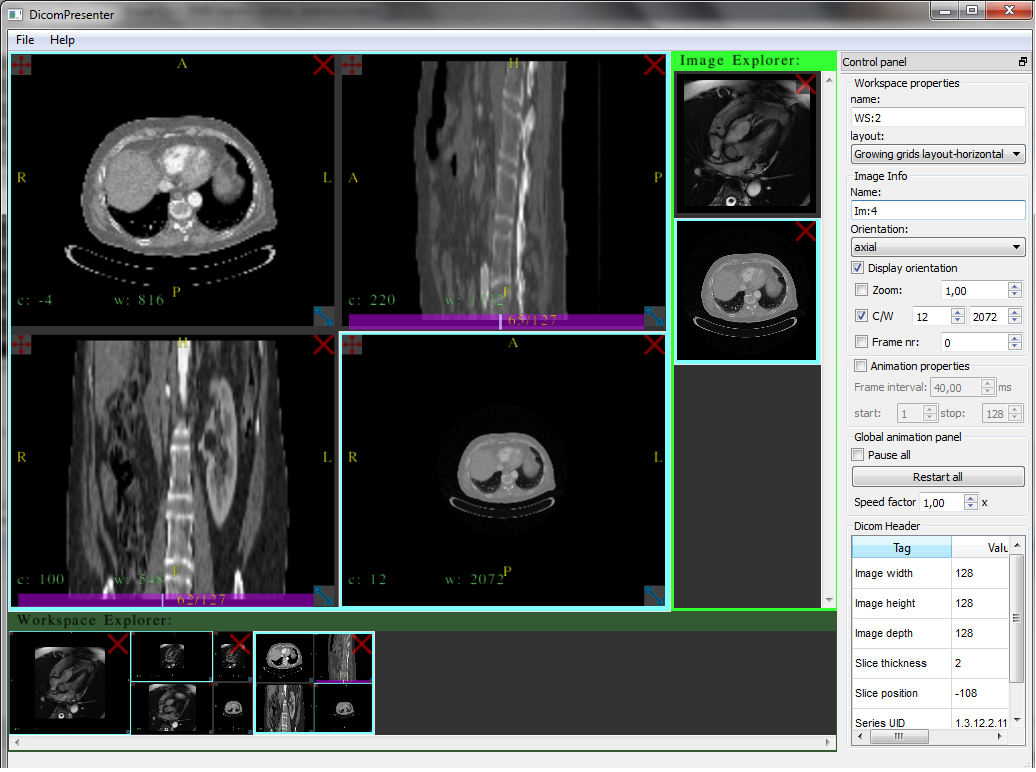
\includegraphics[width=130mm]{Text/IMG/04_GUI_Screenshot.png}
	\end{center}
	\caption{Screenshot of Dicom-Presenter user interface.}
	\label{screenshot}
\end{figure}

\section*{Application requirements}
\addcontentsline{toc}{section}{Application requirements}
The IKEM specialists asked for a typical DICOM images viewer with few more specific features which they missed in freeware programs. A typical DICOM viewer allows you to open .dcm files and display it. .dcm file in this case is a jpeg image equipped with special header including patient information. There you can see a 2D picture of some part of the patient's body. Some DICOM viewers allow you to open series of .dcm files, which can actually fit into a three-dimensional picture. Less commonly it can be a time animation of organ behaviour in short time period (f.e. one heart beat). DICOM viewers often have some more functions but it is very individual.

There have been two more specific requirements on application functionality by IKEM specialists. They missed certain functions in freeware DICOM applications. The most important function was a possibility to open several images at one time and display them on one screen. The user should be allowed to arrange images on screen to any possible layout he prefers. This functionality allows physicians to see two or more different MRI images on screen so they can easily determine pathological differences among observed organs. It is useful for studying, or teaching.

There have been also requirements that the application should be able to record user's manipulation with images as a video. Then physician can prepare his presentation of images at home and then play the video in front of crowds.

\begin{table}[ht]
	\caption{DICOM viewers.}
	\centering
	\begin{tabular}{cc}
			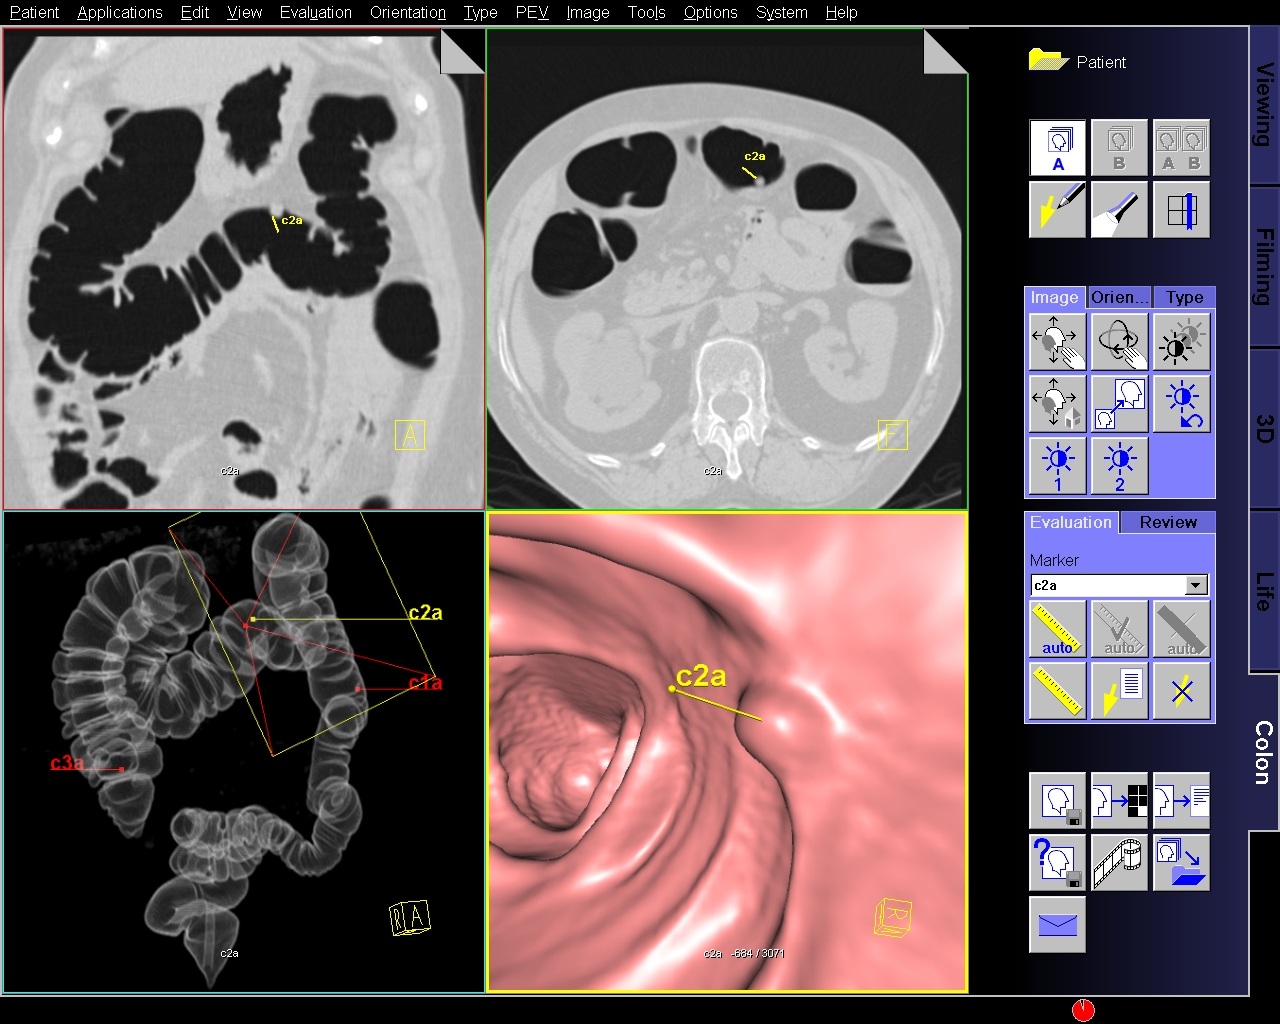
\includegraphics[width=0.5\textwidth,height=0.375\textwidth]{Text/IMG/01_Siemens.jpg}
		&
			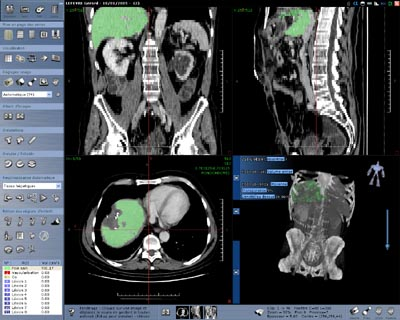
\includegraphics[width=0.5\textwidth,height=0.375\textwidth]{Text/IMG/01_Myrian.jpg}
		\\
			syngo Imaging~\citesec{siemens} & Myrian~\citesec{intrasense}	
		\\
			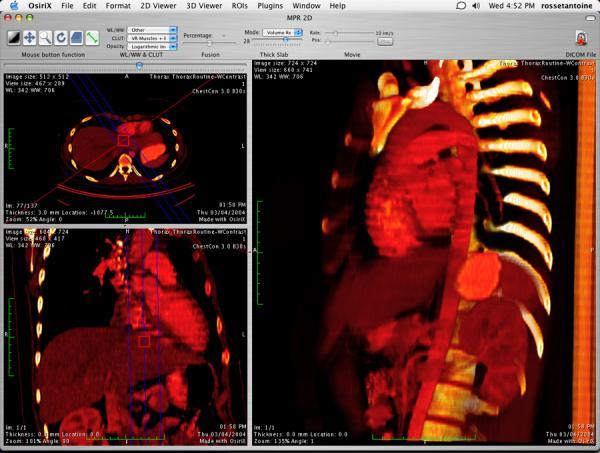
\includegraphics[width=0.5\textwidth,height=0.375\textwidth]{Text/IMG/01_OsiriX.jpg}
		&
			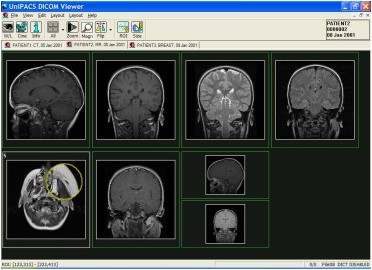
\includegraphics[width=0.5\textwidth,height=0.375\textwidth]{Text/IMG/01_UniPACS.jpg}
		\\
			OsiriX~\citesec{osirix} & UniPACS~\citesec{unipacs}
		\\
		\end{tabular}
\end{table}%
